	\section{Versuchsaufbau und -Durchführung}
	
	\begin{figure}[h!]
		\centering
		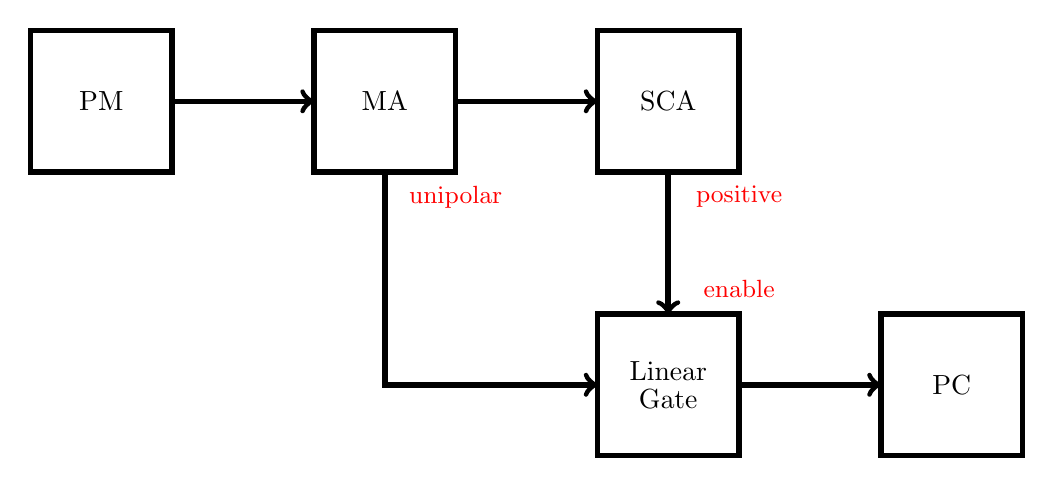
\begin{tikzpicture}[scale=0.9]
		\draw[line width=2] (-1,-1) rectangle (1,1);
		\draw[line width=2] (3,-1) rectangle (5,1);
		\draw[line width=2] (7,-1) rectangle (9,1);
		\draw[line width=2] (7,-5) rectangle (9,-3);
		\draw[line width=2] (11,-5) rectangle (13,-3);
		
		\draw[line width=2,->] (1,0) --(3,0);
		\draw[line width=2,->] (5,0) --(7,0);
		\draw[line width=2,->] (4,-1) --(4,-4) --(7,-4);
		\draw[line width=2,->] (9,-4) --(11,-4);
		\draw[line width=2,->] (8,-1) --(8,-3);
		
		\node at (0,0) {PM};
		\node at (4,0) {MA};
		\node at (8,0) {SCA};
		\node at (8,-3.8) {Linear};
		\node at (8,-4.2) {Gate};
		\node at (12,-4) {PC};
		
		\node[color=red,fill=white] at (5,-1.35) {\small unipolar};
		\node[color=red,fill=white] at (9,-1.35) {\small positive};
		\node[color=red,fill=white] at (9,-2.65) {\small enable};
		
		\end{tikzpicture}
		\caption[Schematische Darstellung des Versuchsaufbaus zum Festlegen des Energiefensters]{Schematische Darstellung des Versuchsaufbaus zum Festelegen des Energiefensters}
		\label{fig:aufbau}
	\end{figure}
	
		
	\begin{figure}[h!]
		\centering
		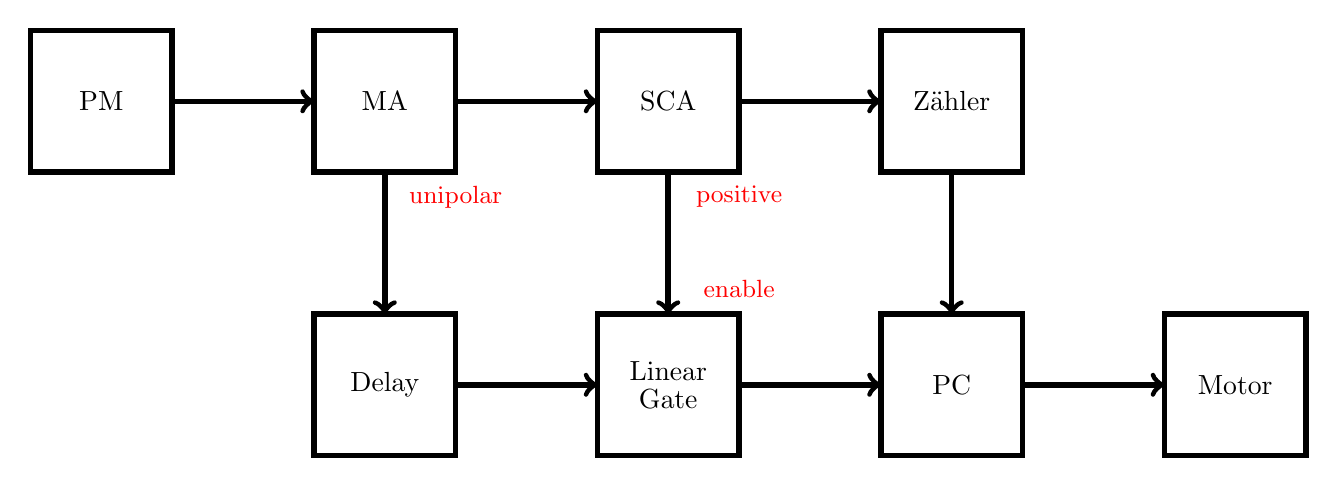
\begin{tikzpicture}[scale=0.9]
		\draw[line width=2] (-1,-1) rectangle (1,1);
		\draw[line width=2] (3,-1) rectangle (5,1);
		\draw[line width=2] (7,-1) rectangle (9,1);
		\draw[line width=2] (11,-1) rectangle (13,1);
		\draw[line width=2] (3,-5) rectangle (5,-3);
		\draw[line width=2] (7,-5) rectangle (9,-3);
		\draw[line width=2] (11,-5) rectangle (13,-3);
		\draw[line width=2] (15,-5) rectangle (17,-3);
		
		\draw[line width=2,->] (1,0) --(3,0);
		\draw[line width=2,->] (5,0) --(7,0);
		\draw[line width=2,->] (9,0) --(11,0);
		\draw[line width=2,->] (5,-4) --(7,-4);
		\draw[line width=2,->] (9,-4) --(11,-4);
		\draw[line width=2,->] (13,-4) --(15,-4);
		\draw[line width=2,->] (4,-1) --(4,-3);
		\draw[line width=2,->] (8,-1) --(8,-3);
		\draw[line width=2,->] (12,-1) --(12,-3);
		
		\node at (0,0) {PM};
		\node at (4,0) {MA};
		\node at (8,0) {SCA};
		\node at (12,0) {Zähler};
		\node at (4,-4) {Delay};
		\node at (8,-3.8) {Linear};
		\node at (8,-4.2) {Gate};
		\node at (12,-4) {PC};
		\node at (16,-4) {Motor};
		
		\node[color=red,fill=white] at (5,-1.35) {\small unipolar};
		\node[color=red,fill=white] at (9,-1.35) {\small positive};
		\node[color=red,fill=white] at (9,-2.65) {\small enable};
		
		\end{tikzpicture}
		\caption[Schematische Darstellung des Versuchsaufbaus]{Schematische Darstellung des Versuchsaufbaus. Hierbei bezeichnet PM den Photomultiplier mit dem Szintillationszähler, MA den Hauptverstärker und SCA den Single Channel Analyzer.}
		\label{fig:aufbau2}
	\end{figure}